\documentclass[twocolumn]{article}
% \setlength{\columnsep}{20pt}
\setlength{\columnseprule}{0.4pt}
\usepackage{v-test-paper}
\renewcommand{\frac}[2]{\dfrac{#1}{#2}}

\begin{document}


\begin{enumerate}
    \item The work function of metal A and B are in the ratio 1:2. If light of frequencies \( f \) and \( 2f \) are incident on the surface of A and B respectively, the ratio of the maximum kinetic energy of photo electrons emitted will be (if \( f \) and \( 2f \) both frequency greater than threshold frequency of metal A and B)
    \begin{tasks}(2)
        \task \( 1 : 1 \)
        \task \( 1 : 2 \)
        \task \( 1 : 3 \)
        \task \( 1 : 4 \)
    \end{tasks}
    \item From the equation \( \tan\theta = \frac{rg}{v^2} \), one can obtain the angle of banking \( \theta \) for a cyclist taking a curve (the symbols have their usual meanings). Then, it is
    \begin{tasks}(1)
        \task Both dimensionally and numerically correct
        \task Neither numerically nor dimensionally correct
        \task Dimensionally correct only
        \task Numerically correct only
    \end{tasks}
    \item The temperature of the two outer surfaces of a compounds slab, each of area \( A \), consisting of two materials having coefficients of thermal conductivity \( K \) and \( 2K \) and thickness \( x \) and \( 4x \), respectively are \( T_2 \) and \( T_1 \) (\( T_2 > T_1 \)). The rate of heat transfer through the slab, in a steady state is \[ \left( \frac{A(T_2 - T_1)K}{x} \right) f, \] with \( f \), which equal to
    \begin{tasks}(2)
        \task \( 1 \)
        \task \( \frac{1}{2} \)
        \task \( \frac{2}{3} \)
        \task \( \frac{1}{3} \)
    \end{tasks}
    \begin{center}
        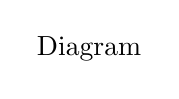
\begin{tikzpicture}
            \node {Diagram};
        \end{tikzpicture}
    \end{center}
    \item A cylinder containing an ideal gas is in vertical position and has a piston of mass \( M \) that is able to move up or down without friction. If the temperature of gas is increased, then
    \begin{tasks}(1)
        \task both pressure and volume of gas will change
        \task Only pressure will increase according to charle's law
        \task Volume will change but not pressure
        \task Pressure will change but not volume
    \end{tasks}
    \begin{center}
        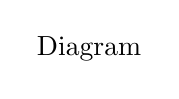
\begin{tikzpicture}
            \node {Diagram};
        \end{tikzpicture}
    \end{center}
    \item A body of mass \( m \) is suspended from a string of length \( l \). What is minimum horizontal velocity that should be given to the body in its lowest position so that it may complete one full revolution in the vertical plane with the point of suspension as the centre of the circle
    \begin{tasks}(2)
        \task \( v = \sqrt{2lg} \)
        \task \( v = \sqrt{3lg} \)
        \task \( v = \sqrt{4lg} \)
        \task \( v = \sqrt{5lg} \)
    \end{tasks}
    \item At \( 27^\circ C \), a gas is suddenly compressed such that its volume becomes \( \frac{1}{8} \)th original volume. Temperature of the gas will be (\( \gamma = \frac{5}{3} \))
    \begin{tasks}(2)
        \task \( 420 \) K
        \task \( 327^\circ C \)
        \task \( 300 \) K
        \task \( 927^\circ C \)
    \end{tasks}
    \item A projectile projected at an angle \( 30^\circ \) from the horizontal has a range \( R \). If the angle of projection at the same initial velocity be \( 60^\circ \), then the range will be
    \begin{tasks}(2)
        \task \( R \)
        \task \( 2R \)
        \task \( \frac{R}{2} \)
        \task \( R^2 \)
    \end{tasks}

    \item On increasing the temperature of a conductor, its resistance increase because
    \begin{tasks}(2)
        \task Relaxation time decreases
        \task Mass of the electrons increases
        \task Electron density decreases
        \task None of these
    \end{tasks}
    \item In the following cyclic process with an ideal gas, during process A $\rightarrow$ B
    \begin{tasks}(1)
        \task Heat is released by the gas
        \task No heat is exchanged
        \task Heat is absorbed by the gas
        \task Work is done on the gas
    \end{tasks}
    \begin{center}
        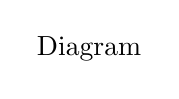
\begin{tikzpicture}
            \node {Diagram};
        \end{tikzpicture}
    \end{center}
    \item C and Si both have the same lattice structure, having 4 bonding electrons in each. However C is insulator whereas Si is intrinsic semiconductor. This is because
    \begin{tasks}(1)
        \task The four bonding electrons in the case of C lie in the second orbit, whereas in the case of Si they lie in the third
        \task The four bonding electrons in the case of C lie in the third orbit, whereas for Si they lie in the fourth orbit
        \task In the case of C, the valence band is not completely filled at absolute zero temperature
        \task In the case of C, the conduction band is partly filled even at absolute zero temperature
    \end{tasks}
    \item Zener diode is used for
    \begin{tasks}(1)
        \task Rectification
        \task Stabilization
        \task Amplification
        \task Producing oscillation in an oscillator
    \end{tasks}
    \item Which represents NOR gate?
    \begin{tasks}(2)
        \task option1.png
        \task option2.png
        \task option3.png
        \task option4.png
    \end{tasks}
    \item To increase the current sensitivity of a moving coil galvanometer, we should
    \begin{tasks}(1)
        \task decrease the number of turns in the coil
        \task decrease the area of cross-section of the coil
        \task increase torsional constant of spiral springs
        \task None of the above
    \end{tasks}
    \item The value of the earth's magnetic field \(B_h = 0.3\) gauss. In this magnetic field, a magnet is oscillating with 5 oscillation/min. To increase the oscillation of the magnet up to 10 oscillation/min, the value of the earth's magnetic field increased by
    \begin{tasks}(2)
        \task 0.3 gauss
        \task 0.6 gauss
        \task 0.9 gauss
        \task 0.12 gauss
    \end{tasks}
    \item A diminished virtual image can be formed only in
    \begin{tasks}(2)
        \task Plane mirror
        \task A concave mirror
        \task A convex mirror
        \task Convex Lens
    \end{tasks}
    \item A thin equiconvex lens has a focal length of 10 cm and a refractive index of 1.5. One of its faces is now silvered, and for an object placed at a distance \(u\) in front of it, the image coincides with the object. The value of \(u\) is
    \begin{tasks}(2)
        \task 10 cm
        \task 5 cm
        \task 20 cm
        \task 15 cm
    \end{tasks}
    \item A solid sphere, a hollow sphere, and a ring are released from the top of an inclined plane (frictionless) so that they slide down the plane. The maximum acceleration down the plane is for (no rolling)
    \begin{tasks}(2)
        \task solid sphere
        \task hollow sphere
        \task ring
        \task all same
    \end{tasks}

    \item A bomb of mass 3m kg explodes into two pieces of mass m kg and 2m kg. If the velocity of m kg mass is 16 m/s, the total kinetic energy released in the explosion is
    \begin{tasks}(2)
        \task 192 mJ
        \task 96 mJ
        \task 384 mJ
        \task 768 mJ
    \end{tasks}

    \item Time period of a satellite in a circular orbit of radius R is `T'. Find the time period of another satellite in a circular orbit of radius 4R
    \begin{tasks}(2)
        \task T
        \task 4 T
        \task 6 T
        \task 8 T
    \end{tasks}

    \item The height upto which water will rise in a capillary tube will be
    \begin{tasks}(1)
        \task Maximum when water temperature is 4$^\circ$C
        \task Maximum when water temperature is 0$^\circ$C
        \task Minimum when water temperature is 4$^\circ$C
        \task Same at all temperatures
    \end{tasks}

    \item An electron and a proton are set free in a uniform electric field the ratio of their acceleration is
    \begin{tasks}(2)
        \task unity
        \task zero
        \task $\frac{m_p}{m_e}$
        \task $\frac{m_e}{m_p}$
    \end{tasks}

    \item A train covers the first half of the distance between two stations with a speed of 40 km/h and the other half with 60 km/h. Then its average speed is
    \begin{tasks}(2)
        \task 50 km/h
        \task 48 km/h
        \task 52 km/h
        \task 100 km/h
    \end{tasks}

    \item An organ pipe $P_1$ closed at one end vibrating in its first overtone and another pipe $P_2$ open at both ends vibrating in its third overtone are in resonance with a given tunning fork. The ratio of the length of $P_1$ to that of $P_2$ is
    \begin{tasks}(2)
        \task 8/3
        \task 3/8
        \task 1/2
        \task 1/3
    \end{tasks}

    \item A suspended long metal wire is stretched a small distance x by a load W in newton suspended at the other end. Select the best answer out of the following
    \begin{tasks}(1)
        \task The loss is potential energy of the load W is equal to the gain in energy of the wire in stretching a length x
        \task The energy stored in the wire can be calculated from the area between the force extension graph and the extension axis
        \task The energy per unit volume stored in the wire $\frac{1}{2} Wx$
        \task None of the above
    \end{tasks}

    \item If the radius of the wire is doubled, then the breaking force If the breaking force for a given wire is F
    \begin{tasks}(2)
        \task 6F
        \task 4F
        \task 8F
        \task F
    \end{tasks}

    \item At what temperature, the mean kinetic energy of $O_2$ will be the same for $H_2$ molecules at -73$^\circ$C
    \begin{tasks}(2)
        \task 127$^\circ$C
        \task 527$^\circ$C
        \task -73$^\circ$C
        \task -173$^\circ$C
    \end{tasks}

    \item In Young's double slit experiment, the 10th maximum of wavelength $\lambda_1$ is at a distance of $y_1$ from the central maximum. When the wavelength of the source is changed to $\lambda_2$, 5th maximum is at a distance of $y_2$ from its central maximum. The ratio $\left(\frac{y_1}{y_2}\right)$ is:
    \begin{tasks}(2)
        \task $\frac{2\lambda_1}{\lambda_2}$
        \task $\frac{2\lambda_2}{\lambda_1}$
        \task $\frac{\lambda_1}{2\lambda_2}$
        \task $\frac{\lambda_2}{2\lambda_1}$
    \end{tasks}

    \item In an oscillating LC circuit the maximum current on the inductor is \( i \). The current in the inductor when the energy is stored equally between the electric and magnetic fields is
    \begin{tasks}(2)
        \task \( \frac{i}{2} \)
        \task \( \frac{i}{\sqrt{3}} \)
        \task \( \frac{i}{\sqrt{2}} \)
        \task \( i \)
    \end{tasks}
    
    \item A coil is suspended in a uniform magnetic field, with the plane of the coil parallel to the magnetic lines of force. When a current is passed through the coil it starts oscillating it is very difficult to stop. But if an aluminium plate is placed near to the coil, stops. This is due to
    \begin{tasks}(1)
        \task Electromagnetic induction in the aluminium plate giving rise to electromagnetic damping
        \task Development of air current when the plate is placed
        \task Induction of electric charge on the plate
        \task Shielding of magnetic lines of force as aluminium is a paramagnetic material
    \end{tasks}
    
    \item Find the angular frequency of particle from given equation: Where \( y = \) displacement and \( t = \) time
    \begin{tasks}(2)
        \task \( \frac{9}{4} \)
        \task \( \frac{4}{9} \)
        \task \( \frac{3}{2} \)
        \task \( \frac{2}{3} \)
    \end{tasks}
    
    \item A car of mass \( 1000 \) kg negotiates a banked curve a radius \( 90 \) m on a frictionless road. If the banking angle is \( 45^\circ \), the speed of the car is
    \begin{tasks}(2)
        \task \( 5 \) ms\(^{-1} \)
        \task \( 10 \) ms\(^{-1} \)
        \task \( 20 \) ms\(^{-1} \)
        \task \( 30 \) ms\(^{-1} \)
    \end{tasks}
    
    \item A voltmeter of resistance \( 1000 \, \Omega \) is connected across a resistance of \( 500 \, \Omega \) in the given circuit. What will be the reading of voltmeter.
    \begin{center}
        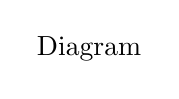
\begin{tikzpicture}
            \node {Diagram};
        \end{tikzpicture}
    \end{center}
    \begin{tasks}(2)
        \task \( 1 \) V
        \task \( 2 \) V
        \task \( 6 \) V
        \task \( 4 \) V
    \end{tasks}
    
    \item A radioactive nucleus of mass \( M \) emits a photon of frequency \( \nu \) and the nucleus recoils. The recoil energy will be :
    \begin{tasks}(2)
        \task \( Mc^2 - h\nu \)
        \task \( \frac{h^2\nu^2}{2Mc^2} \)
        \task zero
        \task \( h\nu \)
    \end{tasks}
    
    \item A spherical portion has been removed from a solid sphere having \( Q \) charge distributed uniformly in its volume as shown in figure. The electric field inside the emptied space is :
    \begin{center}
        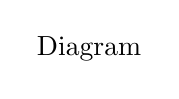
\begin{tikzpicture}
            \node {Diagram};
        \end{tikzpicture}
    \end{center}
    \begin{tasks}(1)
        \task zero energy where
        \task non-zero and uniform
        \task non-uniform
        \task zero only at its centre
    \end{tasks}
    
    \item The flux of the \( \vec{E} \)-field created by the infinitely long wire shown in figure through the spherical gaussian surface of radius \( R \) will be
    \begin{center}
        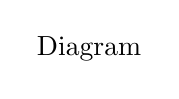
\begin{tikzpicture}
            \node {Diagram};
        \end{tikzpicture}
    \end{center}
    \begin{tasks}(2)
        \task \( \frac{\lambda R}{\varepsilon_0} \)
        \task \( \frac{\sqrt{2}\lambda R}{\varepsilon_0} \)
        \task \( \frac{\sqrt{3}\lambda R}{\varepsilon_0} \)
        \task None.
    \end{tasks}

  \item 
  A current carrying wire LN is bent in th form shown below. If wire carries a current of 10 A and it is placed in a magnetic field of 5T which acts perpendicular to the paper outwards then it will experience a force.
  \begin{tasks}(2)
    \task Zero
    \task 5 N
    \task 30 N
    \task 20 N
  \end{tasks}
  \begin{center}
    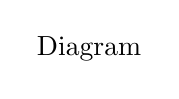
\begin{tikzpicture}
      \node {Diagram};
    \end{tikzpicture}
  \end{center}
  
  \item 
  Susceptibility of Mg at 300 K is \( 1.2 \times 10^{-5} \). The temperature at which susceptibility will be \( 1.8 \times10^{-5} \) is
  \begin{tasks}(2)
    \task 450 K
    \task 200 K
    \task 375 K
    \task None of these
  \end{tasks}
  
  \item 
  A galvanometer has a resistance of \( 3663 \) ohm. A shunt S is connected across it such that \( (1/34) \) of the total current passes through the galvanometer. Then, the value of shunt is:
  \begin{tasks}(2)
    \task 3663 \(\Omega\)
    \task 111 \(\Omega\)
    \task 107.7 \(\Omega\)
    \task 3555.3 \(\Omega\)
  \end{tasks}
  
  \item 
  A ray falls on a prism ABC (AB = BC) and travels as shown in figure. The minimum refractive index of the prism material should be 
  \begin{tasks}(2)
    \task \( \frac{4}{3} \)
    \task \( \sqrt{2} \)
    \task 1.5
    \task \( \sqrt{3} \)
  \end{tasks}
  \begin{center}
    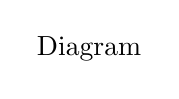
\begin{tikzpicture}
      \node {Diagram};
    \end{tikzpicture}
  \end{center}

  \item 
  A wheel having moment of inertia \( 2 \, \text{kg-m}^2 \) about its vertical axis, rotates at the rate of 60 rpm about the axis. The torque which can stop the wheel’s rotation in one minute would be
  \begin{tasks}(2)
    \task \( \frac{\pi}{12} \, \text{N-m} \)
    \task \( \frac{\pi}{15} \, \text{N-m} \)
    \task \( \frac{\pi}{18} \, \text{N-m} \)
    \task \( \frac{2\pi}{15} \, \text{N-m} \)
  \end{tasks}

  \item Two point charges are kept at a certain distance from one another. The graph represent the variation of the potential along the straight line connecting the two charges.
  \begin{tasks}(1)
    \task \( q_A \) and \( q_B \) both are positive and \( |q_A| > |q_B| \)
    \task \( q_A \) and \( q_B \) both are negative and \( |q_A| < |q_B| \)
    \task Both charges have opposite nature and \( |q_A| > |q_B| \)
    \task Both charges have opposite nature and \( |q_A| < |q_B| \)
  \end{tasks}
  \begin{center}
    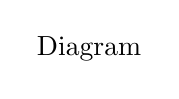
\begin{tikzpicture}
      \node {Diagram};
    \end{tikzpicture}
  \end{center}

  \item 
  The figure shows an instantaneous profile of a rope carrying a progressive wave moving from left to right, then
  \begin{tasks}(1)
    \task (a) the phase at A is greater the phase at B
    \task (b) the phase at B is greater than the phase at A
    \task (c) A is moving upwards
    \task (d) B is moving upwards
  \end{tasks}
  \begin{tasks}(2)
    \task (1) a and c
    \task (2) a and d
    \task (3) b and c
    \task (4) b and d
  \end{tasks}
  \begin{center}
    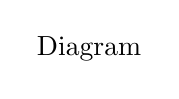
\begin{tikzpicture}
      \node {Diagram};
    \end{tikzpicture}
  \end{center}

  \item 
  Two block of mass 8 kg and 5 kg are connected by a heavy rope of mass 3kg. Complete system is accelerated upwards by \( 10 \, \text{m/s}^2 \) as shown in the figure. The tension at the point ‘P’ will be
  \begin{tasks}(2)
    \task 80 N
    \task 90 N
    \task 160 N
    \task 150 N
  \end{tasks}
  \begin{center}
    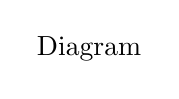
\begin{tikzpicture}
      \node {Diagram};
    \end{tikzpicture}
  \end{center}


    \item A charge \( Q \) is at rest and a person is moving with speed \( v \). The person will feel
    \begin{tasks}(2)
        \task Electric field
        \task Magnetic field
        \task Both 1 and 2
        \task None of the 1 of 2
    \end{tasks}
    \item The potential difference \( V \) and the current \( I \) flowing through an instrument in an ac circuit of frequency \( f \) are given by \( V = 5 \cos \omega t \) volts and \( I = 2 \sin \omega t \) amperes (where \( \omega = 2\pi f \)). The power dissipated in the instrument is
    \begin{tasks}(2)
        \task zero
        \task \(10 \, \text{W}\)
        \task \(5 \, \text{W}\)
        \task \(2.5 \, \text{W}\)
    \end{tasks}
    \item Which of the following relations is correct for an ideal gas?
    \begin{tasks}(2)
        \task \( \gamma - 1 = \frac{f}{2} \)
        \task \( \gamma + 1 = \frac{f}{2} \)
        \task \( \gamma + f = 2 \)
        \task \( \gamma + f = 3 \)
    \end{tasks}
    \item Assertion: For a capacitor, charge stored is given as \( Q = CV \) \\
    Reason: Capacitance of a capacitor is independent of charging voltage.
    \begin{tasks}(1)
        \task If both assertion and reason are true and the reason is the correct explanation of the assertion
        \task If both assertion and reason are true but reason is not the correct explanation of the assertion
        \task If assertion is true but reason is false
        \task If the assertion and reason both are false
    \end{tasks}
    \item A wire of resistance \( 5 \, \Omega \) connected to a battery of potential \( 10 \, \text{V} \). The current flow in the wire is
    \begin{tasks}(2)
        \task \(5 \, \text{A}\)
        \task \(4 \, \text{A}\)
        \task \(2 \, \text{A}\)
        \task \(1 \, \text{A}\)
    \end{tasks}
    \item Two identical capacitors each of capacitance are \( 5\mu \text{F} \) charged to potential \( 2 \text{kV} \) and \( 1 \text{kV} \) respectively. The \(-\)ve ends are connected together. When the \(+\)ve ends are also connected together, the loss of energy of the system is
    \begin{tasks}(2)
        \task \(160 \, \text{J}\)
        \task \(0 \, \text{J}\)
        \task \(5 \, \text{J}\)
        \task \(1.25 \, \text{J}\)
    \end{tasks}
    \item As shown in the figure, a magnet is moved with a fast speed towards a coil at rest. Due to this induced electromotive force, induced current, and induced charge in the coil are \( E \), \( I \), and \( Q \) respectively. If the speed of the magnet is doubled, the incorrect statement is:
    \begin{tasks}(2)
        \task \( E \) increases
        \task \( I \) increases
        \task \( Q \) remains the same
        \task \( Q \) increases
    \end{tasks}
    \begin{center}
        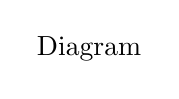
\begin{tikzpicture}
            \node {Diagram};
        \end{tikzpicture}
    \end{center}

    \item Given below are two statements : \\
    Statement I : Acetophenone shows aldol condensation \\
    Statement II : Acetophenone contains Carbonyl group \\
    In the light of the above statements, choose the most appropriate answer from the options given below :
    \begin{tasks}(1)
        \task Both Statement I and Statement II are incorrect
        \task Statement I is correct but Statement II is incorrect
        \task Statement I is incorrect but Statement II is correct
        \task Both Statement I and Statement II are correct
    \end{tasks}
    
    \item Assertion: \\
    \centerline{
    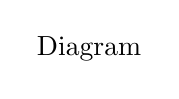
\begin{tikzpicture}
        \node {Diagram};
    \end{tikzpicture}
    }
    Reason: In hydroboration-oxidation no carbocation intermediate is formed and BH$_3$ acts as an electrophile because of empty P orbital on B. \\
    In the light of the above statements, choose the most appropriate answer from the options given below:
    \begin{tasks}(1)
        \task Both (A) and (R) are correct but (R) is not the correct explanation of (A)
        \task (A) is correct but (R) is not correct
        \task (A) is not correct but (R) is correct
        \task Both (A) and (R) are correct and (R) is the correct explanation of (A)
    \end{tasks}
    
    \item Which one is the correct order of acidity:
    \begin{tasks}(1)
        \task CH$_3$-CH$_3$ > CH$_2$=CH$_2$ > CH$_3$-C$\equiv$CH > CH$\equiv$CH
        \task CH$_3$-CH$_2$CH$_3$ > CH$_3$-CH$_2$-CH$_2$-CH$_3$ > CH$_3$-C$\equiv$CH > CH$\equiv$CH
        \task CH$\equiv$CH-CH$_3$ > C$\equiv$CH > CH$_2$=CH-CH$_2$-CH$_3$ > CH$_3$-CH$_3$
        \task CH$\equiv$CH-CH$_2$ > CH$_3$ > CH-CH$_2$ > CH$_3$-C$\equiv$CH-CH$_3$
    \end{tasks}
    
    \item In which pair of ions both the species contains S-S bond:
    \begin{tasks}(1)
        \task S$_4$O$_6$$^{2-}$, S$_2$O$_7$$^{2-}$
        \task S$_2$O$_7$$^{2-}$, S$_2$O$_8$$^{2-}$
        \task S$_4$O$_6$$^{2-}$, S$_2$O$_3$$^{2-}$
        \task S$_2$O$_7$$^{2-}$, S$_2$O$_6$$^{2-}$
    \end{tasks}
    
    \item Decreasing order of stability of O$_2$, O$_2$$^-$, O$_2$$^+$ and O$_2$$^{2-}$ is:
    \begin{tasks}(1)
        \task O$_2$$^{2-}$ > O$_2$ > O$_2$$^+$ > O$_2$$^-$
        \task O$_2$ > O$_2$$^+$ > O$_2$$^{2-}$ > O$_2$$^-$
        \task O$_2$$^+$ > O$_2$ > O$_2$$^{2-}$ > O$_2$$^-$
        \task O$_2$$^+$ > O$_2$ > O$_2$$^-$ > O$_2$$^{2-}$
    \end{tasks}
    
    \item In which option properties of the given three complex are correct:
    \begin{tasks}(1)
        \task Square planar     Paramagnetic     $\mu = \sqrt{8}$ BM
        \task $\mu = 0$         tetrahedral      diamagnetic
        \task diamagnetic       $\mu = \sqrt{8}$ BM         Square planar
        \task Square planar     Diamagnetic      Tetrahedral
    \end{tasks}
    
    \item Match the metal ions given in Column I with the spin magnetic moments of the ions given in Column II and assign the correct code:
    \begin{tabular}{p{5cm}p{5cm}}
        \textbf{Column I} & \textbf{Column II} \\
        a. Co$^{3+}$  & i. $\sqrt{8}$ B.M. \\
        b. Cr$^{3+}$  & ii. $\sqrt{35}$ B.M. \\
        c. Fe$^{3+}$  & iii. $\sqrt{3}$ B.M. \\
        d. Ni$^{2+}$  & iv. $\sqrt{24}$ B.M. \\
                     & v. $\sqrt{15}$ B.M.
    \end{tabular}
    \begin{tasks}(2)
        \task a-iii, b-v, c-i, d-ii
        \task a-iv, b-v, c-ii, d-i
        \task a-iv, b-i, c-ii, d-iii
        \task a-i, b-ii, c-iii, d-iv
    \end{tasks}
    
    \item Reaction BaO$_2$(s) $\rightleftharpoons$ BaO(s) + O$_2$(g); $\Delta H = +ve$. In equilibrium condition pressure of O$_2$ depends on:
    \begin{tasks}(1)
        \task Increase mass of BaO$_2$
        \task Increase mass of BaO
        \task Increase temperature on equilibrium
        \task Increase mass of BaO$_2$ and BaO both
    \end{tasks}
    
    \item For the redox reaction \\
    MnO$_4$$^-$ + C$_2$O$_4$$^{2-}$ + H$^+ \rightarrow$ Mn$^{2+}$ + CO$_2$ + H$_2$O \\
    the correct coefficients of the reactants for the balanced equation are:
    \begin{tasks}(1)
        \task MnO$_4$$^-$ 5, C$_2$O$_4$$^{2-}$ 16, H$^+$ 2
        \task MnO$_4$$^-$ 2, C$_2$O$_4$$^{2-}$ 16, H$^+$ 5
        \task MnO$_4$$^-$ 5, C$_2$O$_4$$^{2-}$ 16, H$^+$ 2
        \task MnO$_4$$^-$ 2, C$_2$O$_4$$^{2-}$ 5, H$^+$ 16
    \end{tasks}

    \item In the above reaction major product \& mechanism is:
    \begin{tasks}(2)
        \task CH$_3$I, SN$^1$
        \task CH$_3$I,SN$^2$
        \task PhI,SN$^1$
        \task PhI,SN$^2$
    \end{tasks}
    \item For a reaction A $\rightarrow$ 2B, rate of disappearance of `A' is related to the rate of appearance of `B' by the expression:
    \begin{tasks}(2)
        \task $-\dfrac{d[A]}{dt} = 4 \dfrac{d[B]}{dt}$
        \task $-\dfrac{d[A]}{dt} = \dfrac{1}{2} \dfrac{d[B]}{dt}$
        \task $-\dfrac{d[A]}{dt} = \dfrac{1}{4} \dfrac{d[B]}{dt}$
        \task $-\dfrac{d[A]}{dt} = d[B]$
    \end{tasks}
    \item In the following sequence of reactions, the compound `B' will be:
    \begin{tasks}(2)
        \task CH$_3$CHO
        \task CH$_3$CH$_2$CHO
        \task CH$_3$COCH$_3$
        \task CH$_3$CH$_2$COCH$_3$
    \end{tasks}
    \item Which of the following relations is correct?
    \begin{tasks}(2)
        \task $K_3 \cdot K^3_2 = K^2_1$
        \task $K_1 \cdot \sqrt{K_2} = K_3$
        \task $K_1 \cdot K_3 = K_1$
        \task $K_3 = K_1 \cdot K_2$
    \end{tasks}
    \item The state of hybridization of carbons 1, 3 and 5 are in the following sequence:
    \begin{tasks}(2)
        \task sp, sp$^3$, sp$^2$
        \task sp, sp$^2$, sp$^3$
        \task sp$^3$, sp$^2$, sp
        \task sp$^2$, sp, sp$^3$
    \end{tasks}
    \item In which case in number of molecule of water maximum:
    \begin{tasks}(1)
        \task 18 mL of water
        \task 0.18 gm of water
        \task 0.00224 It of water vapour at 1 atm and 273 K
        \task $10^{-3}$ mole of water
    \end{tasks}
    \item The conjugate acid of NH$_2^-$ is:
    \begin{tasks}(2)
        \task NH$_3$
        \task NH$_2$OH
        \task NH$^+$
        \task N$_2$H$_4$
    \end{tasks}
    \item The structure of intermediate A in the following reaction is:
    % The image depicts chemical structures which require a different approach to be represented in LaTeX, likely through a package like chemfig or mhchem. In this case, we represent it as a Diagram node.
    \begin{center}
        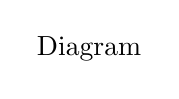
\begin{tikzpicture}
            \node {Diagram};
        \end{tikzpicture}
    \end{center}
    \item Which of the following gives iodoform test:
    \begin{tasks}(2)
        \task CH$_3$CHO
        \task HCHO
        \task Both
        \task None
    \end{tasks}

    \item The pH of 0.01 M NaOH solution will be : 
    \begin{tasks}(2)
        \task 7.01
        \task 2
        \task 12
        \task 9
    \end{tasks}
    
    \item Which one of the following ions exhibits d-d transition and para magnetism as will be :
    \begin{tasks}(2)
        \task $\text{CrO}_4^{-2}$
        \task $\text{Cr}_2\text{O}_7^{-2}$
        \task $\text{MnO}_4^{-}$
        \task $\text{MnO}_4^{-2}$
    \end{tasks}
    
    \item For the cell reaction
    \[2\text{Fe}^{3+} (aq) + 2\text{I}^- (aq) \rightarrow 2\text{Fe}^{2+} (aq) + \text{I}_2(aq)\]
    \[E^\circ_{\text{cell}} = 0.24\ V \text{ at } 298\ K\]
    The standard Gibbs energy ($\Delta G^\circ$) of the cell reaction is:
    \[\text{[Given that Faraday constant } F = 96500\ C\ mol^{-1}]\]
    \begin{tasks}(2)
        \task $-46.32\ kJ\ mol^{-1}$
        \task $-23.16\ kJ\ mol^{-1}$
        \task $46.32\ kJ\ mol^{-1}$
        \task $23.16\ kJ\ mol^{-1}$
    \end{tasks}
    
    \item The IUPAC name of the compound is :
    \begin{center}
        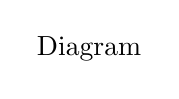
\begin{tikzpicture}
            \node {Diagram};
        \end{tikzpicture}
    \end{center}
    \begin{tasks}(1)
        \task 5-Methylhex-3-en-2-ol
        \task 2-Methylhex-3-en-5-ol
        \task 2-Hydroxy-5-methyl-3-hexene
        \task 5-Hydroxy-2-methyl-3-hexene
    \end{tasks}
    
    \item During the formation of a chemical bond :
    \begin{tasks}(1)
        \task Energy of the system does not change
        \task Electron-electron repulsion becomes more than the nucleus-electron attraction
        \task Energy decreases
        \task Energy increases
    \end{tasks}
    
    \item Which of the following polymers is prepared by addition polymerisation :
    \begin{tasks}(2)
        \task Dacron
        \task Teflon
        \task Nylon-6,6
        \task Novolac
    \end{tasks}
    
    \item Name and Catalyst of the following reaction is :
    \begin{center}
        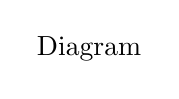
\begin{tikzpicture}
            \node {Diagram};
        \end{tikzpicture}
    \end{center}
    \begin{tasks}(1)
        \task Stephen reaction – $\text{H}_2 + \text{Pd/BaSO}_4$
        \task Rosenmund reduction – $\text{SnCl}_4/\text{HCl}+\text{H}_3\text{O}^+$
        \task Rosenmund reduction – $\text{H}_2+\text{Pd} – \text{BaSO}_4$
        \task Etard reaction – $\text{CrO}_2\text{Cl}_2/\text{CS}_2$
    \end{tasks}
    
    \item If 0.5 mol of $\text{BaCl}_2$ is mixed with 0.2 mol $\text{Na}_3\text{PO}_4$, then maximum number of moles of $\text{Ba}_3(\text{PO}_4)_2$ that can be formed is :
    \begin{tasks}(2)
        \task 0.7
        \task 0.5
        \task 0.3
        \task 0.1
    \end{tasks}
    
    \item The $t_{1/2}$ of first order reaction is :
    \begin{tasks}(1)
        \task dependent upon initial concentration
        \task directly proportional to initial concentration
        \task indirectly proportional to initial concentration
        \task independent of initial concentration
    \end{tasks}
    
    \item All real gases behaves as ideal under-
    \begin{tasks}(1)
        \task low pressure, high temperature
        \task high pressure, high temperature
        \task low pressure, low temperature
        \task high pressure, low temperature
    \end{tasks}
    
    \item Standard electrode potentials of two half cells are given as
    \[\text{Zn}^{2+}/\text{Zn} = -0.76\ V\]
    \[\text{Ag}^+/\text{Ag} = 0.80\ V\]
    The EMF of the cell
    \[\text{Zn}|\text{Zn}^{2+} (1M) || \text{Ag}^+ (1M) | \text{Ag}\]
    will be :
    \begin{tasks}(2)
        \task 1.56 V
        \task 1.20 V
        \task 0.04 V
        \task -1.56 V
    \end{tasks}

    \item The correct order of acidic strength is :
    \begin{tasks}(1)
        \task \( \mathrm{CH_3CF_2COOH > CH_3CCl_2COOH > CH_3CBr_2COOH} \)
        \task \( \mathrm{CH_3CF_2COOH > CH_3CBr_2COOH > CH_3CCl_2COOH} \)
        \task \( \mathrm{CH_3CBr_2COOH > CH_3CCl_2COOH > CH_3CF_2COOH} \)
        \task \( \mathrm{CH_3CCl_2COOH > CH_3CBr_2COOH > CH_3CF_2COOH} \)
    \end{tasks}
    
    \item In test for primary amines, the amine is treated with CHCl\(_3\) and KOH and a bad smelling compound is formed. If the primary amine used is ethylamine, identify the bad smelling compound formed:
    \begin{tasks}(2)
        \task \( \mathrm{CH_3CN} \)
        \task \( \mathrm{CH_3CNO} \)
        \task \( \mathrm{CH_3CH_2NC} \)
        \task \( \mathrm{CH_3NCO} \)
    \end{tasks}
    
    \item CaC\(_2\) + H\(_2\)O \(\rightarrow\) A \( \overset{\mathrm{H_2SO_4}}{\rightarrow} \) B \( \overset{\mathrm{HgSO_4}}{\rightarrow} \)
    Identify A and B in the above reaction:
    \begin{tasks}(1)
        \task \( \mathrm{C_2H_2} \) and \( \mathrm{CH_3COOH} \)
        \task \( \mathrm{C_2H_4} \) and \( \mathrm{CH_3COOH} \)
        \task \( \mathrm{CH_4} \) and \( \mathrm{HCOOH} \)
        \task \( \mathrm{C_2H_2} \) and \( \mathrm{CH_3CHO} \)
    \end{tasks}

    \item Which of the following sets of quantum numbers is not correct:
    \begin{tasks}(1)
        \task \( n = 2 \), \( l = 0 \), \( m = 0 \), \( s = +\frac{1}{2} \)
        \task \( n = 4 \), \( l = 3 \), \( m = 2 \), \( s = +\frac{1}{2} \)
        \task \( n = 2 \), \( l = 2 \), \( m = 0 \), \( s = -\frac{1}{2} \)
        \task All of these
    \end{tasks}
    
    \item Which of the following is most stable:
    \begin{tasks}(2)
        \task \( \mathrm{Sn^{2+}} \)
        \task \( \mathrm{Ge^{2+}} \)
        \task \( \mathrm{Si^{2+}} \)
        \task \( \mathrm{Pb^{2+}} \)
    \end{tasks}
    
    \item Order of stability
    \begin{center}
        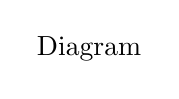
\begin{tikzpicture}
            \node {Diagram};
        \end{tikzpicture}
    \end{center}
    \begin{tasks}(2)
        \task \( \mathrm{Z > X > Y} \)
        \task \( \mathrm{X > Y > Z} \)
        \task \( \mathrm{Y > Z > X} \)
        \task \( \mathrm{X > Z > Y} \)
    \end{tasks}
    
    \item Which one of the following substances has the highest proton affinity:
    \begin{tasks}(2)
        \task \( \mathrm{H_2O} \)
        \task \( \mathrm{H_2S} \)
        \task \( \mathrm{NH_3} \)
        \task \( \mathrm{PH_3} \)
    \end{tasks}
    
    \item If the ground state energy of a one electron species is \(-E_0\), then the wavelength of light emitted if an electron jumps from \(3^\text{rd}\) excited state to ground state will be
    \begin{tasks}(2)
        \task \( \frac{hc}{E_0} \)
        \task \( \frac{5E_0}{2hc} \)
        \task \( \frac{9hc}{8E_0} \)
        \task \( \frac{16hc}{15E_0} \)
    \end{tasks}
    
    \item 12.3 g nitrobenzene is reduced into aniline by electrolysis, if current efficiency is 25\% calculate charge reduced in coulombs:
    \begin{tasks}(1)
        \task \( 12 \times 96500 \) coulombs
        \task \( 1.2 \times 9650 \) coulombs
        \task \( 24 \times 9650 \) coulombs
        \task \( 96500 \) coulombs
    \end{tasks}
    
    \item In the preparation of compounds of Xe, Bartlett had taken \( \mathrm{O_2^+}\cdot\mathrm{PtF_6^-} \) as a base compound. This is because:
    \begin{tasks}(1)
        \task Both \( \mathrm{O_2} \) and Xe have same size
        \task Both \( \mathrm{O_2} \) and Xe have same electron gain enthalpy
        \task Both \( \mathrm{O_2} \) and Xe have almost same ionisation enthalpy
        \task Both Xe and \( \mathrm{O_2} \) are gases
    \end{tasks}

    \item The correct order of acidic strength is :
    \begin{tasks}(1)
        \task \( \mathrm{CH_3CF_2COOH > CH_3CCl_2COOH > CH_3CBr_2COOH} \)
        \task \( \mathrm{CH_3CF_2COOH > CH_3CBr_2COOH > CH_3CCl_2COOH} \)
        \task \( \mathrm{CH_3CBr_2COOH > CH_3CCl_2COOH > CH_3CF_2COOH} \)
        \task \( \mathrm{CH_3CCl_2COOH > CH_3CBr_2COOH > CH_3CF_2COOH} \)
    \end{tasks}
    
    \item In test for primary amines, the amine is treated with CHCl\(_3\) and KOH and a bad smelling compound is formed. If the primary amine used is ethylamine, identify the bad smelling compound formed:
    \begin{tasks}(2)
        \task \( \mathrm{CH_3CN} \)
        \task \( \mathrm{CH_3CNO} \)
        \task \( \mathrm{CH_3CH_2NC} \)
        \task \( \mathrm{CH_3NCO} \)
    \end{tasks}
    
    \item CaC\(_2\) + H\(_2\)O \(\rightarrow\) A \( \overset{\mathrm{H_2SO_4}}{\rightarrow} \) B \( \overset{\mathrm{HgSO_4}}{\rightarrow} \)
    Identify A and B in the above reaction:
    \begin{tasks}(1)
        \task \( \mathrm{C_2H_2} \) and \( \mathrm{CH_3COOH} \)
        \task \( \mathrm{C_2H_4} \) and \( \mathrm{CH_3COOH} \)
        \task \( \mathrm{CH_4} \) and \( \mathrm{HCOOH} \)
        \task \( \mathrm{C_2H_2} \) and \( \mathrm{CH_3CHO} \)
    \end{tasks}

    \item Which of the following sets of quantum numbers is not correct:
    \begin{tasks}(1)
        \task \( n = 2 \), \( l = 0 \), \( m = 0 \), \( s = +\frac{1}{2} \)
        \task \( n = 4 \), \( l = 3 \), \( m = 2 \), \( s = +\frac{1}{2} \)
        \task \( n = 2 \), \( l = 2 \), \( m = 0 \), \( s = -\frac{1}{2} \)
        \task All of these
    \end{tasks}
    
    \item Which of the following is most stable:
    \begin{tasks}(2)
        \task \( \mathrm{Sn^{2+}} \)
        \task \( \mathrm{Ge^{2+}} \)
        \task \( \mathrm{Si^{2+}} \)
        \task \( \mathrm{Pb^{2+}} \)
    \end{tasks}
    
    \item Order of stability
    \begin{center}
        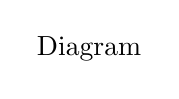
\begin{tikzpicture}
            \node {Diagram};
        \end{tikzpicture}
    \end{center}
    \begin{tasks}(2)
        \task \( \mathrm{Z > X > Y} \)
        \task \( \mathrm{X > Y > Z} \)
        \task \( \mathrm{Y > Z > X} \)
        \task \( \mathrm{X > Z > Y} \)
    \end{tasks}
    
    \item Which one of the following substances has the highest proton affinity:
    \begin{tasks}(2)
        \task \( \mathrm{H_2O} \)
        \task \( \mathrm{H_2S} \)
        \task \( \mathrm{NH_3} \)
        \task \( \mathrm{PH_3} \)
    \end{tasks}
    
    \item If the ground state energy of a one electron species is \(-E_0\), then the wavelength of light emitted if an electron jumps from \(3^\text{rd}\) excited state to ground state will be
    \begin{tasks}(2)
        \task \( \frac{hc}{E_0} \)
        \task \( \frac{5E_0}{2hc} \)
        \task \( \frac{9hc}{8E_0} \)
        \task \( \frac{16hc}{15E_0} \)
    \end{tasks}
    
    \item 12.3 g nitrobenzene is reduced into aniline by electrolysis, if current efficiency is 25\% calculate charge reduced in coulombs:
    \begin{tasks}(1)
        \task \( 12 \times 96500 \) coulombs
        \task \( 1.2 \times 9650 \) coulombs
        \task \( 24 \times 9650 \) coulombs
        \task \( 96500 \) coulombs
    \end{tasks}
    
    \item In the preparation of compounds of Xe, Bartlett had taken \( \mathrm{O_2^+}\cdot\mathrm{PtF_6^-} \) as a base compound. This is because:
    \begin{tasks}(1)
        \task Both \( \mathrm{O_2} \) and Xe have same size
        \task Both \( \mathrm{O_2} \) and Xe have same electron gain enthalpy
        \task Both \( \mathrm{O_2} \) and Xe have almost same ionisation enthalpy
        \task Both Xe and \( \mathrm{O_2} \) are gases
    \end{tasks}

    \item Which among the given molecules can exhibit tautomerism:

    \begin{center}
    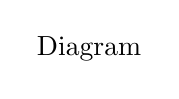
\begin{tikzpicture}
        \node {Diagram};
    \end{tikzpicture}
    \end{center}

    \begin{tasks}(2)
        \task Cyclohexane
        \task Cyclohexanone
        \task Phenol
        \task Both 2 and 3
    \end{tasks}

    \item Which one of the following is the incorrect match?
    \begin{tasks}(1)
        \task Mollusch – Branchial respiration
        \task Fish – Gills
        \task Mammals – Pulmonary respiration
        \task Mollusch – Only pulmonary respiration
    \end{tasks}
    \item Heart $\rightarrow$ deoxygenated blood $\rightarrow$ gills $\rightarrow$ oxygenated blood $\rightarrow$ body parts $\rightarrow$ deoxygenated blood $\rightarrow$ heart. This is
    \begin{tasks}(1)
        \task Single circulation
        \task Incomplete double circulation
        \task Double circulation
        \task None of these
    \end{tasks}
    \item Given below are two statements
    
    Statement I:
    
    The efferent arteriole emerging from the glomerulus forms a fine capillary network around the renal tubule called the peritubular capillaries.
    
    Statement II:
    
    Vasa recta is absent or highly reduced in cortical nephrons.
    
    Choose the correct answer from the option given below:
    \begin{tasks}(1)
        \task Both Statement I and Statement II are incorrect
        \task Statement I is correct but Statement II is incorrect
        \task Statement I is incorrect but Statement II is correct
        \task Both Statement I and Statement II are correct
    \end{tasks}
    \item The given diagram is: \\
    \begin{center}
        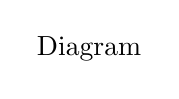
\begin{tikzpicture}
            \node {Diagram};
        \end{tikzpicture}
    \end{center}
    \begin{tasks}(2)
        \task Meromyosin
        \task Myosin monomer
        \task Acting filament
        \task Both 1 and 2
    \end{tasks}
    \item Select the correct option for the given diagram: \\
    \begin{center}
        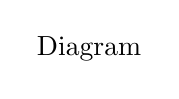
\begin{tikzpicture}
            \node {Diagram};
        \end{tikzpicture}
    \end{center}
    \begin{tasks}(2)
        \task A–Cranial bone
        \task B–Facial bone
        \task E–Facial bone
        \task All
    \end{tasks}
    \item How many are chlorophyll bearing organism:
    \begin{tasks}(2)
        \task 7
        \task 6
        \task 8
        \task 10
    \end{tasks}
    \item Select the correct route for the passage of sperms in male frogs.
    \begin{tasks}(1)
        \task Testes $\rightarrow$ Bidder’s canal $\rightarrow$ Kidney $\rightarrow$ Vasa efferentia $\rightarrow$ Urogenital duct $\rightarrow$ Cloaca
        \task Testes $\rightarrow$ Vasa efferentia $\rightarrow$ Kidney $\rightarrow$ Seminal vesicle $\rightarrow$ Urogenital duct $\rightarrow$ Cloaca
        \task Testes $\rightarrow$ Vasa efferentia $\rightarrow$ Bidder’s canal $\rightarrow$ Ureter $\rightarrow$ Cloaca
        \task Testes $\rightarrow$ Vasa efferentia $\rightarrow$ Kidney $\rightarrow$ Bidder’s canal $\rightarrow$ Urogenital duct $\rightarrow$ Cloaca
    \end{tasks}
    \item Frog's heart when taken out of the body continues to beat for some time. Select the option containing the correct statements.
    \begin{tasks}(1)
        \task Only III
        \task Only IV
        \task I and II
        \task III and IV
    \end{tasks}

    \item In which of the following options are incorrect:
    \begin{tasks}(2)
        \task Only a, b
        \task Only a, c
        \task Only a, d
        \task Only c, d
    \end{tasks}
    
    \item The given below diagram of animal belongs to
    \begin{tasks}(2)
        \task Reptilia
        \task Chordata
        \task Urochordata
        \task All
    \end{tasks}
    \begin{center}
        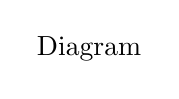
\begin{tikzpicture}
            \node {Diagram};
        \end{tikzpicture}
    \end{center}
    
    \item The given below diagram is
    \begin{tasks}(2)
        \task Tape worm
        \task Chindoblast
        \task Sycon
        \task Octopus
    \end{tasks}
    \begin{center}
        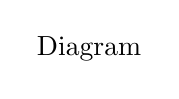
\begin{tikzpicture}
            \node {Diagram};
        \end{tikzpicture}
    \end{center}

    \item The given floral formula related to which plant:
    \begin{tasks}(2)
        \task Gloriosa
        \task Mustard
        \task Tomato
        \task Soyabean
    \end{tasks}
    
    \item In which of the following plants Bisexual flower present:
    \begin{tasks}(2)
        \task Tulip
        \task Sesbania
        \task China rose
        \task All
    \end{tasks}
    
    \item Which of the following is not a function of the skeletal system:
    \begin{tasks}(1)
        \task Production of body heat
        \task Locomotion
        \task Production of erythrocytes
        \task Storage of minerals
    \end{tasks}
    
    \item Ground tissue includes:
    \begin{tasks}(1)
        \task all tissues except epidermis and vascular bundles
        \task epidermis and cortex
        \task all tissues internal to endodermis
        \task all tissues external to endodermis
    \end{tasks}
    
    \item Continuous wavy ring cambium formed in
    \begin{tasks}(2)
        \task Monocot root
        \task Dicot root
        \task Monocot stem
        \task Dicot stem
    \end{tasks}
    
    \item Study the four statements (i-iv) given below and select the two correct ones out of them.
    \begin{tasks}(2)
        \task (ii) and (iii)
        \task (iii) and (iv)
        \task (i) and (iv)
        \task (i) and (ii).
    \end{tasks}

    \item Which of the following organisms in the given food web act as a secondary consumer?
    \begin{center}
        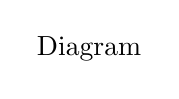
\begin{tikzpicture}
            \node {Diagram};
        \end{tikzpicture}
    \end{center}
    \begin{tasks}(2)
        \task I and IV
        \task V and VI
        \task III and VI
        \task IV and VII
    \end{tasks}

    \item The German naturalist and geographer Alexander von Humboldt observed that within a region species richness increased with increasing explored area, but only up to a limit. In fact, relation between species richness and area for a wide variety of taxa (angiosperm plants, birds, bats, freshwater fishes) turns out to be rectangular hyperbola. Now find out correct equations shown in the graph.
    \begin{center}
        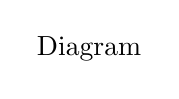
\begin{tikzpicture}
            \node {Diagram};
        \end{tikzpicture}
    \end{center}
    \begin{tasks}(1)
        \task I: \( S = CA^{Z} \); II: \( \log S = \log C + Z \log A \)
        \task I: \( \log S = \log C + Z \log A \); II: \( S - CA^{Z} \)
        \task I: \( S - CA^{Z} \) + \( \log C \); II: \( \log S = \log C + Z \log A \)
        \task I: \( S - CA^{Z} \) + \( \log A \); II: \( \log S = \log C + Z \log A \)
    \end{tasks}

    \item Select the correct option for the given diagram.
    \begin{center}
        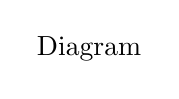
\begin{tikzpicture}
            \node {Diagram};
        \end{tikzpicture}
    \end{center}
    \begin{tasks}(1)
        \task A-Desert
        \task B-Tropical forest
        \task C-Temperate forest
        \task D-Arctic and alpine tundra
    \end{tasks}

    \item Match the Column I with Column II with respect to the nomenclature of enzyme Eco RI and select the correct answer from codes given below.
    % Omitted tabular environment for matching.

    \item How many are example of Exsitu - conservation
    \begin{tasks}(1)
        \task Zoological park
        \task National park
        \task Wild life safari park
        \task Botanical garden
        \task Sacred groves
    \end{tasks}
    \begin{tasks}(2)
        \task Two
        \task Three
        \task Four
        \task One
    \end{tasks}

    \item Which one of the following contains minimum content of energy:
    \begin{tasks}(2)
        \task Grass
        \task Snake
        \task Grasshopper
        \task Frogs
    \end{tasks}

    \item An Individual has certain attributes. This attributes are:
    \begin{tasks}(5)
        \task Death
        \task Birth
        \task Death rate
        \task Birth rate
        \task Sex ratio
    \end{tasks}
    \begin{tasks}(2)
        \task \(a, b\)
        \task \(c, d, e\)
        \task Only \(e\)
        \task Only \(c, d\)
    \end{tasks}

    \item If \(20 \, J\) of energy is trapped at producer level, then how much energy will be available to peacock as food in the following food chain?
    \begin{tasks}(2)
        \task \(0.02 \, J\)
        \task \(0.002 \, J\)
        \task \(0.2 \, J\)
        \task \(0.0002 \, J\)
    \end{tasks}

    %% solution for above question
    

    \item Given below is the diagram of the ecological pyramids.
          \begin{center}
              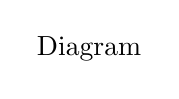
\begin{tikzpicture}
                  \node {Diagram};
              \end{tikzpicture}
          \end{center}
          This type represents
          \begin{tasks}(1)
              \task pyramid of number in a grassland
              \task pyramid of biomass in a lake
              \task pyramid of biomass in a land
              \task pyramid of energy
          \end{tasks}
    \item In the given below diagram identify A, B, C, D:
          \begin{center}
              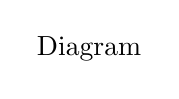
\begin{tikzpicture}
                  \node {Diagram};
              \end{tikzpicture}
          \end{center}
          \begin{tasks}(2)
              \task A -- Angiosperm
              \task B -- Mosses
              \task C -- Ferns and allies
              \task D -- Lichens
          \end{tasks}
    \item Which one of the following are maximum number of species in Amazonian Rain forest
          \begin{tasks}(2)
              \task Plants
              \task Amphibians
              \task Invertebrates
              \task Fishes
          \end{tasks}
    \item The pelvic girdle consists of:
          \begin{tasks}(1)
              \task Two scapula and one clavicle
              \task Two scapula and two clavicle
              \task One scapula and one coxal bone
              \task Two coxal bone
          \end{tasks}
    \item Given below are two statements
          \begin{tasks}(1)
              \task Both Statement I and Statement II are incorrect
              \task Statement I is correct but Statement II is incorrect
              \task Statement I is incorrect but Statement II is correct
              \task Both Statement I and Statement II are correct
          \end{tasks}
    \item Given below are two statements
          \begin{tasks}(1)
              \task Both Statement I and Statement II are incorrect
              \task Statement I is correct but Statement II is incorrect
              \task Statement I is incorrect but Statement II is correct
              \task Both Statement I and Statement II are correct
          \end{tasks}
    \item The exaggerated response of the immune system to certain antigens present in the environment is called
          \begin{tasks}(2)
              \task Immunity
              \task Passive immunity
              \task Innate immunity
              \task Allergy
          \end{tasks}
    \item Injury localised to the hypothalamus would most likely to disrupt
          \begin{tasks}(1)
              \task short term memory
              \task coordination during locomotion
              \task executive function, such as decision making
              \task regulation of body temperature
          \end{tasks}
    \item Given below are two statements
          \begin{tasks}(1)
              \task Both Statement I and Statement II are incorrect
              \task Statement I is correct but Statement II is incorrect
              \task Statement I is incorrect but Statement II is correct
              \task Both Statement I and Statement II are correct
          \end{tasks}
    \item Given below are two statements
          \begin{tasks}(1)
              \task Both Statement I and Statement II are incorrect
              \task Statement I is correct but Statement II is incorrect
              \task Statement I is incorrect but Statement II is correct
              \task Both Statement I and Statement II are correct
          \end{tasks}
    \item Given below are two statements
          \begin{tasks}(1)
              \task Both Statement I and Statement II are incorrect
              \task Statement I is correct but Statement II is incorrect
              \task Statement I is incorrect but Statement II is correct
              \task Both Statement I and Statement II are correct
          \end{tasks}
    \item In \textit{E. coli}, during lactose metabolism, in absence of inducer, repressor protein binds to:
          \begin{tasks}(2)
              \task Regulator gene
              \task Operator
              \task Structural gene
              \task Promoter
          \end{tasks}
    \item Given below are two statements
          \begin{tasks}(1)
              \task Both Statement I and Statement II are incorrect
              \task Statement I is correct but Statement II is incorrect
              \task Statement I is incorrect but Statement II is correct
              \task Both Statement I and Statement II are correct
          \end{tasks}
    \item If a sample of B-DNA contains 100000 Nucleosome then what is the length of B-DNA sample:
          \begin{tasks}(2)
              \task 0.68 mm
              \task 6.8 mm
              \task 0.68 cm
              \task Both 2 and 3
          \end{tasks}
    \item Corn borer is controlled by protein encoded by gene
          \begin{tasks}(2)
              \task cryIAc
              \task cryIAb
              \task Both 1 and 2
              \task None of these
          \end{tasks}
    \item The primers used during annealing step of PCR are
          \begin{tasks}(1)
              \task Polypeptides
              \task A type of nucleic acids
              \task Lipids
              \task Carbohydrates
          \end{tasks}

    \item Thermostable DNA polymerase is taq polymerase. Taq are related with
    \begin{tasks}(2)
        \task Virus
        \task Fungi
        \task Bacteria
        \task Plant
    \end{tasks}
    \item How many matching are correct :
    \begin{tasks}(1)
        \task Natural Genetic Engineer - \textit{E.coli}
        \task Natural Genetic Engineer - \textit{Agrobacterium}
        \task Plasmid - Extra chromosomal DNA
        \task Alkaline pH - Required for activation of Bt Toxin
    \end{tasks}
    \begin{tasks}(4)
        \task Three
        \task Four
        \task Two
        \task One
    \end{tasks}
    \item How many matching are correct :
    \begin{tasks}(1)
        \task \text{ELi Lilly} - Indian company
        \task \text{ELi Lilly} - Formation of Human insulin
        \task Pro-Insulin - A - Peptide
        \task Pro-Insulin - B - Peptide
    \end{tasks}
    \begin{tasks}(2)
        \task Three
        \task Four
        \task Two
        \task One
    \end{tasks}
    \item Transgenic animals may be useful for
    \begin{tasks}(1)
        \task Study of normal physiology and development
        \task Study of disease
        \task Producing biological products
        \task All of the above
    \end{tasks}
    \item 'The integration of natural science and organisms cells, parts there of, and molecular analogues for products and services'
    
    Above given sentence is
    \begin{tasks}(1)
        \task Definition of bioinformatics
        \task Definition of biotechnology
        \task Special method of tissue culture
        \task Special method for hybridisation
    \end{tasks}
    \item Given below are two statements
    
    Statement I:
    
    Some plasmids may have only one or two copies per cell whereas others may have 15--100 copies per cell.
    
    Statement II :
    
    Plasmids and Bacteriophage have the ability to replicate within bacterial cell independent of the control of chromosomal DNA.
    
    Choose the correct answer from the option given
    below:
    
    \begin{tasks}(1)
        \task Both Statement I and Statement II are incorrect
        \task Statement I is correct but Statement II is incorrect
        \task Statement I is incorrect but Statement II is correct
        \task Both Statement I and Statement II are correct
    \end{tasks}
    \item Which one of the following is wrong statement :
    \begin{tasks}(1)
        \task Phosphorus is a constituent of cell membranes, certain nucleic acids and all proteins
        \task \textit{Nitrosomonas} and \textit{Nitrobacter} are chemoautotrophs
        \task \textit{Anabaena} and \textit{Nostoc} are capable of fixing nitrogen in free-living state also
        \task Root nodule forming nitrogen fixers live as aerobes under free-living conditions.
    \end{tasks}
    \item Select the correct option for the given reaction
    
    \begin{center}
        \[\text{N} \equiv \text{N} \quad \stackrel{\text{X}}{\longrightarrow} \quad \text{NH}_3\]
    \end{center}
    
    \begin{tasks}(1)
        \task X is nitrogenase
        \task X present in prokaryotes
        \task X related with nitrogen metabolism
        \task All
    \end{tasks}
    \item Which one of the following 4-carbon containing compound forms in mesophyll cells :
    
    \begin{tasks}(2)
        \task OAA
        \task Malic acid
        \task Aspartic acid
    \end{tasks}
    \begin{tasks}(2)
        \task Only a
        \task Only a, b
        \task Only a, c
        \task All of these
    \end{tasks}
    \item Which of the following is true During photosynthesis
    \begin{tasks}(1)
        \task Several factors interact and simultaneously effect photosynthesis
        \task Usually one factor is the major cause and limit the rate
        \task At any point the rate will be determined by the factor available at suboptimal levels
        \task All of these are true
    \end{tasks}
    \item What is not true about bundle sheath cells of maize:
    \begin{tasks}(1)
        \task They have numerous chloroplast
        \task Intercellular spaces absent
        \task Their walls are not impervious to gaseous exchange
        \task Their walls are thick
    \end{tasks}
    \item Which one of the following is correct match for pollen grain
    \begin{tasks}(1)
        \task Exine - Inner layer
        \task Intine - Outer layer
        \task Exine - Continuous layer
        \task Intine - Made up of pectin and cellulose
    \end{tasks}
    \item Which one of the following is the correct match for fruits
    \begin{tasks}(1)
        \task Fleshy - Papaya
        \task Dry - Groundnuts
        \task Parthenocarpic - Seed less
        \task All
    \end{tasks}
    \item Which one of the following is not related with ovule of flowering plant
    \begin{tasks}(1)
        \task Middle layers
        \task Nucellus
        \task Embryo sac
        \task Micropylar pole
    \end{tasks}
    \item Late blight of potato is caused by :
    \begin{tasks}(1)
        \task Bacteria
        \task Virus
        \task Fungus
        \task Protozoa
    \end{tasks}
    \item Biopesticides are
    \begin{tasks}(1)
        \task The chemicals which are used to destroy the pests
        \task The living organism or their products which are used for pest control
        \task The organisms which destroy the crops
        \task None of these
    \end{tasks}
    \item Select the correct statement for the given diagram
    \begin{center}
        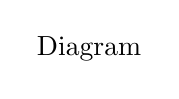
\begin{tikzpicture}
            \node {Diagram};
        \end{tikzpicture}
    \end{center}
    \begin{tasks}(1)
        \task Related with hershey and Chase
        \task Related with E. coli
        \task It is represents semiconservative replication
        \task Heavy isotope used
    \end{tasks}
    \begin{tasks}(2)
        \task All
        \task b, c, d
        \task a, b, c
        \task Only c, d
    \end{tasks}
    \item Which of the following disease is not an air borne disease
    \begin{tasks}(1)
        \task Pneumonia
        \task Filariasis
        \task Common cold
        \task None of these
    \end{tasks}
    \item Select the correct option for the given diagram
    \begin{center}
        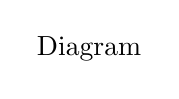
\begin{tikzpicture}
            \node {Diagram};
        \end{tikzpicture}
    \end{center}
    \begin{tasks}(1)
        \task Stabilising type of natural selection
        \task Disruptive type of natural selection
        \task Directional type of natural selection
        \task None of these
    \end{tasks}
    \item Which one of the following are not a extinct animal
    \begin{tasks}(1)
        \task Brachiosaurus
        \task Stegosaurus
        \task Pelycosaurus
        \task None of these
    \end{tasks}

    \item Which one of the following hormones is involved in sugar metabolism?
        \begin{tasks}(2)
            \task Insulin
            \task Glucagon
            \task Cortisone
            \task All
        \end{tasks}
    \item Given below are two statements\\
    Statement I: Closely located genes assorted together and distantly located genes, due to recombination assorted independently.\\
    Statement II: Many genes were linked to sexes also and called sex-linked genes.\\
    Choose the correct answer from the option given below:
        \begin{tasks}(1)
            \task Both Statement I and Statement II are incorrect
            \task Statement I is correct but Statement II is incorrect
            \task Statement I is incorrect but Statement II is correct
            \task Both Statement I and Statement II are correct
        \end{tasks}
    \item Given below are two statements\\
    Statement I: In down syndrome palm is broad with characteristic palm crease.\\
    Statement II: In down syndrome and klinefelter syndrome number of chromosome are same.\\
    Choose the correct answer from the option given below:
        % Same tasks environment as above, with respective statements.
        \begin{tasks}(1)
            \task Both Statement I and Statement II are incorrect
            \task Statement I is correct but Statement II is incorrect
            \task Statement I is incorrect but Statement II is correct
            \task Both Statement I and Statement II are correct
        \end{tasks}
    \item Given below are two statements\\
    Statement I: The thalassemia could be due to either mutation or deletion which ultimately results in reduced rate of synthesis of one of the globin chains (\(\alpha\) and \(\beta\) chains) that make up haemoglobin.\\
    Statement II: Due to haemophilia in an affected individual a simple cut will result in non-stop bleeding.\\
    Choose the correct answer from the option given below:
        % Same tasks environment as above, with respective statements.
        \begin{tasks}(1)
            \task Both Statement I and Statement II are incorrect
            \task Statement I is correct but Statement II is incorrect
            \task Statement I is incorrect but Statement II is correct
            \task Both Statement I and Statement II are correct
        \end{tasks}
    \item Given below are two statements\\
    Statement I: In addition to recombination, mutation is another phenomenon that leads to variation in DNA.\\
    Statement II : UV radiation can cause mutation in organisms. It is a mutagen.\\
    Choose the correct answer from the option given below:
        % Same tasks environment as above, with respective statements.
    \item Given below are two statements\\
    Statement I: Deletions and insertions of base pairs of DNA, causes frame - shift mutations.\\
    Statement II : In honey bee the number of chromosome in queen and worker are same.\\
    Choose the correct answer from the option given below:
        % Same tasks environment as above, with respective statements.
        \begin{tasks}(1)
            \task Both Statement I and Statement II are incorrect
            \task Statement I is correct but Statement II is incorrect
            \task Statement I is incorrect but Statement II is correct
            \task Both Statement I and Statement II are correct
        \end{tasks}
    \item Given below are two statements\\
    Statement I: Further investigation by other scientist led to the conclusion that the X-body of henking was in fact a chromosome and that is why it was given the name X-chromosome.\\
    Statement II : Today genetic maps are extensively used as a starting point in the sequencing of whole genomes as was done in the case of the human genome sequencing project, describe later.\\
    Choose the correct answer from the option given below:
        % Same tasks environment as above, with respective statements.
        \begin{tasks}(1)
            \task Both Statement I and Statement II are incorrect
            \task Statement I is correct but Statement II is incorrect
            \task Statement I is incorrect but Statement II is correct
            \task Both Statement I and Statement II are correct
        \end{tasks}
    \item Given below are two statements\\
    Statement I: Platelets also called thrombocytes are cell fragments produced from megakaryocytes.\\
    Statement II : Platelets are involved in the coagulation of blood.\\
    Choose the correct answer from the option given below:
        % Same tasks environment as above, with respective statements.
        \begin{tasks}(1)
            \task Both Statement I and Statement II are incorrect
            \task Statement I is correct but Statement II is incorrect
            \task Statement I is incorrect but Statement II is correct
            \task Both Statement I and Statement II are correct
        \end{tasks}
    \item Assertion (A): The Human Heart are myogenic type\\
    Reason (R): In Human Heart intercalated disc are present\\
    Choose the correct answer from the option given below:
        \begin{tasks}(1)
            \task Both (A) and (R) are true but (R) is not the correct explanation of (A)
            \task (A) is true but (R) is false
            \task (A) is false but (R) is true
            \task Both (A) and (R) are true and (R) is the correct explanation of (A)
        \end{tasks}
    \item The process of oxidative phosphorylation takes place in :
        \begin{tasks}(2)
            \task Mitochondria
            \task Chloroplasts
            \task Ribosomes
            \task Cytoplasm
        \end{tasks}
    \item Which is the connecting link between glycolysis and Kreb's cycle :
        \begin{tasks}(2)
            \task Iso-citric acid
            \task \(\alpha\)-ketoglutaric acid
            \task Glucose
            \task Acetyl Co-A
        \end{tasks}
    \item Consider the statements as True/False regarding when a neuron is at rest and no impulse is conducting.\\
    I. The axoplasm inside the axon contains high concentration of K\(^+\) and negatively charged proteins.\\
    II. The axoplasm inside the axon contains low concentration of Na\(^+\).\\
    III. The fluid outside the axon contains a low concentration of K\(^+\).\\
    IV. The fluid outside the axon contains a low concentration of Na\(^+\) and negatively charged proteins.\\
    The correct option is
        \begin{tasks}(1)
            \task True \quad False \quad False \quad True
            \task True \quad True \quad False \quad False
            \task True \quad True \quad True \quad False
            \task False \quad True \quad False \quad False
        \end{tasks}
    \item In tissue \(pO_2\) and \(pCO_2\) are respectively :
        \begin{tasks}(1)
            \task 45 mmHg and 40 mmHg
            \task 40 mmHg and 45 mmHg
            \task 40 mmHg and 40 mmHg
            \task 45 mmHg and 45 mmHg
        \end{tasks}
    \item How many fragments will be generated, if a closed circular DNA molecule is digested using a restriction enzyme having six recognition sites on the DNA?
        \begin{tasks}(4)
            \task 4
            \task 6
            \task 7
            \task 5
        \end{tasks}
    \item If the sequence of m-RNA is AUGUUUCUUUAUUUAUCU Then what is the sequence of amino acid in polypeptide chain :
        \begin{tasks}(1)
            \task met-Phe-Leu-Ile-Ile-Ser
            \task met-Leu-Phe-Ile-Ile-Ser
            \task met-Leu-Ile-Phe-Ile-Ser
            \task met-Phe-Leu-Ile-Ser-Ile
        \end{tasks}
    \item Given below are two statements\\
    Statement I: The mammary glands of the female undergo differentiation during pregnancy and starts producing milk towards the end of pregnancy by the process called lactation.\\
    Statement II : The milk produced during the initial few days of lactation is called colostrum.\\
    Choose the correct answer from the option given below:
        % Same tasks environment as above, with respective statements.
        \begin{tasks}(1)
            \task Both Statement I and Statement II are incorrect
            \task Statement I is correct but Statement II is incorrect
            \task Statement I is incorrect but Statement II is correct
            \task Both Statement I and Statement II are correct
        \end{tasks}
    \item Given below are two statements\\
    Statement I: Lymph is also an important carrier for nutrients and Hormones.\\
    Statement II : Fats are absorbed through lymph in the lacteals present in the Intestinal villi.\\
    Choose the correct answer from the option given below:
        % Same tasks environment as above, with respective statements.

    % \item Choose the correct answer from the option given below:
    \begin{tasks}(1)
        \task Both Statement I and Statement II are incorrect
        \task Statement I is correct but Statement II is incorrect
        \task Statement I is incorrect but Statement II is correct
        \task Both Statement I and Statement II are correct
    \end{tasks}
    
    
   
  

    \item Which disease is related to the discovery of gibberellins:
    \begin{tasks}(2)
        \task Minamata disease
        \task Citrus canker
        \task Bakane disease
        \task Black rot of cabbage
    \end{tasks}

    \item In human male reproductive system, secretion of which gland constitute the seminal plasma:
    \begin{tasks}(1)
        \task Paired seminal vesicle, paired prostate, a bulbourethral gland
        \task Paired seminal vesicle, a prostate, a bulbourethral gland
        \task A seminal vesicle, paired prostate, paired bulbourethral gland
        \task Paired seminal vesicle, a prostate, paired bulbourethral gland
    \end{tasks}

    \item Study the following statements regarding chemiosmotic hypothesis in mitochondria.
    \begin{enumerate}
        \item \(F_1\) head-piece contains the site for the synthesis of ATP from ADP + Pi.
        \item \(F_o\) part forms the channel through which protons cross the inner membrane.
        \item The passage of protons through the channel is coupled to the catalytic site of the \(F_1\) component for the ATP production.
        \item For each ATP produced, 2H\(^+\) pass through \(F_o\) from the intermembrane space to the matrix against the electrochemical process gradient.
    \end{enumerate}
    Select the option depicting the correct statements.
    \begin{tasks}(2)
        \task 1 and II
        \task I, II and III
        \task 1 and III
        \task I, II, III and IV
    \end{tasks}

    \item In mycorrhiza function of hyphae:
    \begin{tasks}(1)
        \task Protection of algae
        \task Absorb mineral ion and water from soil
        \task In photosynthesis
        \task All of these
    \end{tasks}

    \item In Calvin cycle, if one molecule of RuBP is carboxylated than how many PGA molecule will be formed?
    \begin{tasks}(2)
        \task 2
        \task 3
        \task 4
        \task 5
    \end{tasks}

    \item Recombination is completed in which phase of meiosis:
    \begin{tasks}(2)
        \task Leptotene
        \task Zygotene
        \task Pachytene
        \task Diakinesis
    \end{tasks}

    \item Which one of the following event are not related with meiosis I
    \begin{tasks}(1)
        \task Splitting of centromere
        \task Synapsis
        \task Cytokinesis
        \task Recombination
    \end{tasks}

    \item In oocytes of some vertebrates which stage can last for months or years
    \begin{tasks}(2)
        \task Diplotene
        \task Pachytene
        \task Diakinesis
        \task Leptotene
    \end{tasks}

    \item Select the correct option, which represents the homopolysaccharides made up of glucose monomers:
    \begin{tasks}(1)
        \task Sucrose, lactose, maltose
        \task Chitin, glycogen, starch
        \task Starch, inulin, peptidoglycan
        \task Starch, glycogen, cellulose
    \end{tasks}

    \item Which one of the following is not correct regarding the endomembrane system:
    \begin{tasks}(1)
        \task Formed by those organelles whose functions are well coordinated
        \task It consist of endoplasmic reticulum, microbodies and peroxisome
        \task It consist of endoplasmic reticulum, golgi complex, lysosome and vacuoles
        \task Both 1 and 3
    \end{tasks}

    \item What is the NAD and NADP:
    \begin{tasks}(1)
        \task Coenzyme
        \task Cofactor
        \task Vitamin containing chemical
        \task All
    \end{tasks}

    \item Which of the following cells do not have nucleus at maturity:
    \begin{tasks}(2)
        \task Mature erythrocytes
        \task Sieve tube cells
        \task Both 1 and 2
        \task Lysosome
    \end{tasks}

    \item A leaves have surface area 10 cm\(^2\) after some time due to growth their surface area increased and finally 15 cm\(^2\). What is the \% of relative growth rate:
    \begin{tasks}(2)
        \task 25 \%
        \task 50 \%
        \task 33.3 \%
        \task 66.6 \%
    \end{tasks}

    \item Generally after fertilisation the sepals, petals and stamens of the flower:
    \begin{tasks}(1)
        \task Wither and fall off
        \task Grow and become enlarged
        \task No clear idea about this
        \task Colour become changed
    \end{tasks}

    \item A common character of dicot stem and dicot root is
    \begin{tasks}(1)
        \task Exarch protoxylem
        \task Endarch protoxylem
        \task Occurrence of secondary growth
        \task All
    \end{tasks}

    \item In which plants the gametophytic phase represented by single to few celled haploid gametophyte
    \begin{tasks}(2)
        \task Sphagnum
        \task Spirogyra
        \task Sequoia
        \task Salvinia
    \end{tasks}

    \item Sporophytic generation is represented only by the one celled zygote. There are no free living sporophytes. Meiosis in the zygote results in the formation of haploid spores. This kind of life cycles is termed as:
    \begin{tasks}(1)
        \task Haplo-diplontic
        \task Haplontic
        \task Diplontic
        \task May be diplontic or haplontic
    \end{tasks}

    \item Which one of the following is correct statement
    \begin{tasks}(1)
        \task ABA act as an antagonistics to auxin
        \task ABA act as an antagonistics to GA
        \task Ethylene is also called stress hormone
        \task GA stimulates the closure of stomata
    \end{tasks}

    \item The BSE is
    \begin{tasks}(1)
        \task Bacillus special encephalopathy
        \task Bovine special encephalopathy
        \task Bovine spongiform encephalopathy
        \task Bovine sterile encephalopathy
    \end{tasks}

    \item \textit{Eucalyptus}, \textit{Sphagnum}, \textit{Ginkgo}, \textit{Sequoia}, \textit{Polysiphonia}, \textit{Selaginella}, \textit{Pteris}.
    How many members have pollen grain:
    \begin{tasks}(2)
        \task 6
        \task 4
        \task 5
        \task 3
    \end{tasks}

    \item Given below are two statements
    \begin{description}
        \item[Statement I:] A fertile stamens is called staminode
        \item[Statement II:] When stamens are attached to the sepals, they are called epipetalous as in brinjal.
    \end{description}
    Choose the correct answer from the option given below:
    \begin{tasks}(1)
        \task Both Statement I and Statement II are incorrect
        \task Statement I is correct but Statement II is incorrect
        \task Statement I is incorrect but Statement II is correct
        \task Both Statement I and Statement II are correct
    \end{tasks}

    \item In laboratory a scientist working on human cells culture, He observed on a single human cells then after 10 days how many human cells are formed through division in laboratory:
    \begin{tasks}(2)
        \task 2048
        \task 4096
        \task 512
        \task 1024
    \end{tasks}
\end{enumerate}



\end{document}